\subsection{Primeiros protótipos}

Um dos processos de desenvolvimento de uma Aplicação Web é a criação de protótipos (\emph{Mockups}) que demonstrem de como será o aspeto visual da nossa aplicação.\\
Durante a produção dos primeiros protótipos, teve-se como objetivo identificar de que formas as várias funcionalidades do sistemas iriam estar presentes na aplicação, sem haver preocupações com questões estéticas.Este protótipos foram desenvolvidos usanto a aplicação \href{http://balsamiq.com/products/mockups/}{\emph{Balsamiq Mockups}}(Figura ~\ref{fig: balsamiq}).\\

\begin{figure}[htbp] 
        \centering
        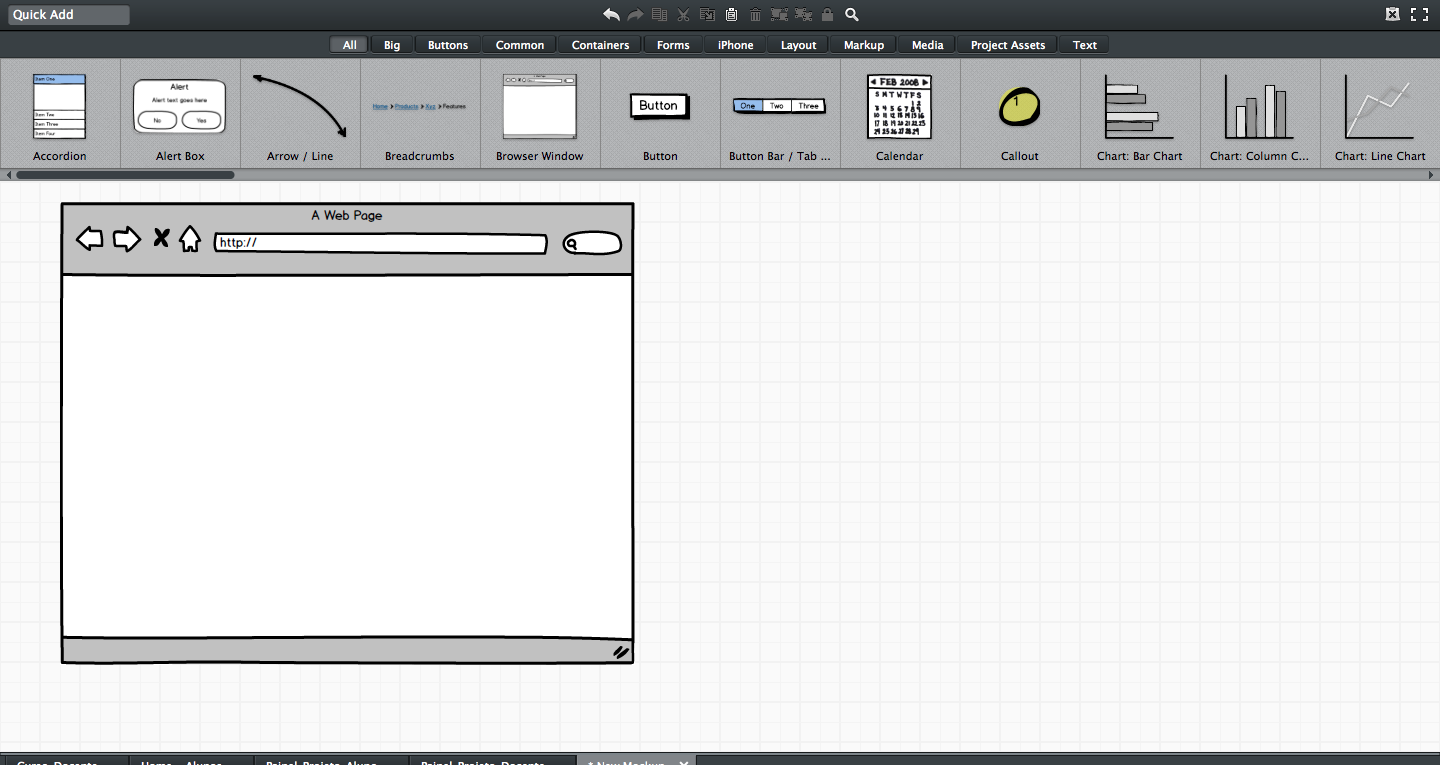
\includegraphics[width=1\textwidth]{images/prototipos/mockups/balsamiq.png}
         \caption{\emph{Balsamiq Mockups}}
         \label{fig: balsamiq}
\end{figure}


%Introdução a falar dos mockups feitos
Sobre os prótipos feitos, teve-se como preocupação a simplicidade da pagina, a quantidade de informação e o tempo de navegação, isto é a quantidade de ações que um utilizador tem que fazer para passar de uma página para outra.\\
Começando pela página inicial (Figura ~\ref{fig: home}) está mostra as várias funcionalidades da aplicação, fazendo a distinção entre alunos e docentes.Também é possivel aceder aos projetos públicos do sistema.\\

\begin{figure}[htbp] 
        \centering
        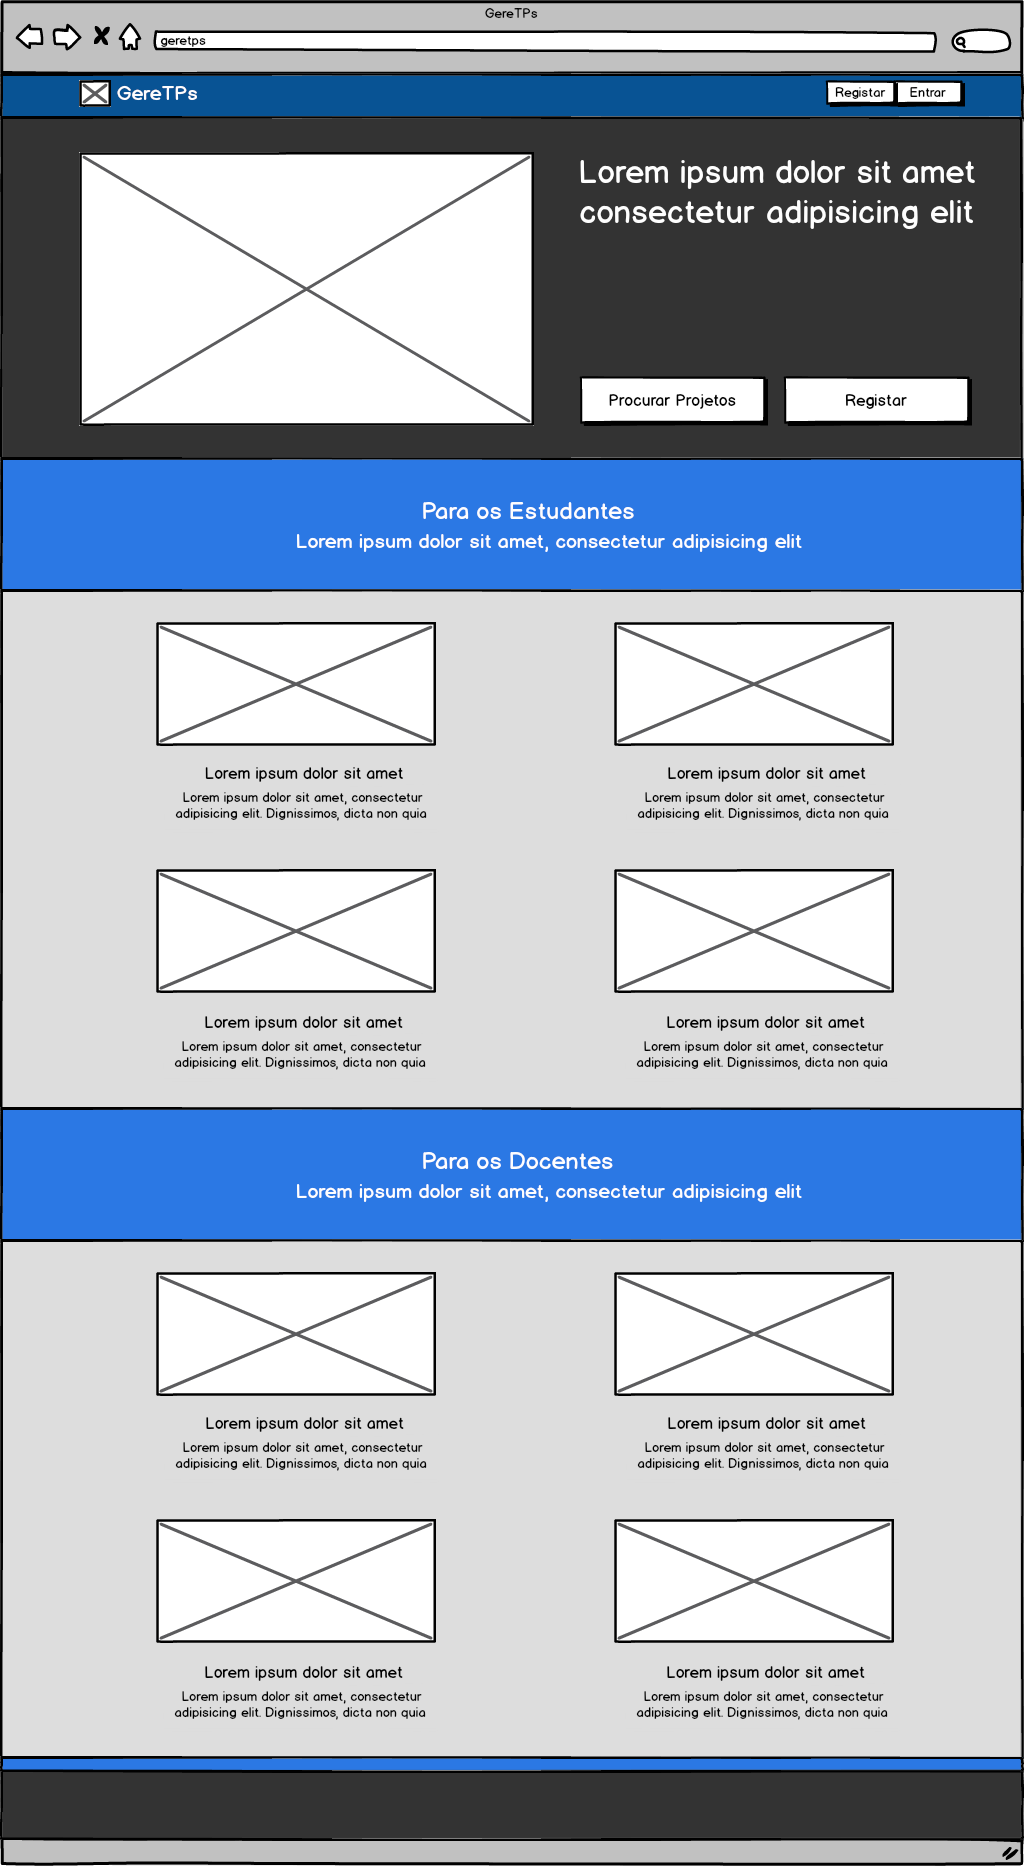
\includegraphics[width=1\textwidth]{images/prototipos/mockups/home.png}
         \caption{Página inicial}
         \label{fig: home}
\end{figure}

No painel de uma disciplina(Figura ~\ref{fig: cursodocente}), um docente pode ter acesso aos últimos acontecimentos dentro das disciplina, sabendo quando aconteceram submissões nos projetos desta, assim alterações da mesma.Também existem informações sobre os projetos criados na disciplina, no qual são apresentadas informações sobre o nome do prjeto, número de fases,estado e número de entregas até ao momento. No caso de ser o docente responsável da disciplina podes adicionar professores de forma direta sem que haja a necessidade de abrir formulários adicionais e fazer gestão de turnos. Caso contrário apenas poderá ver o estado dos turnos e quais são os docentes da disciplina.\\

\begin{figure}[htbp] 
        \centering
        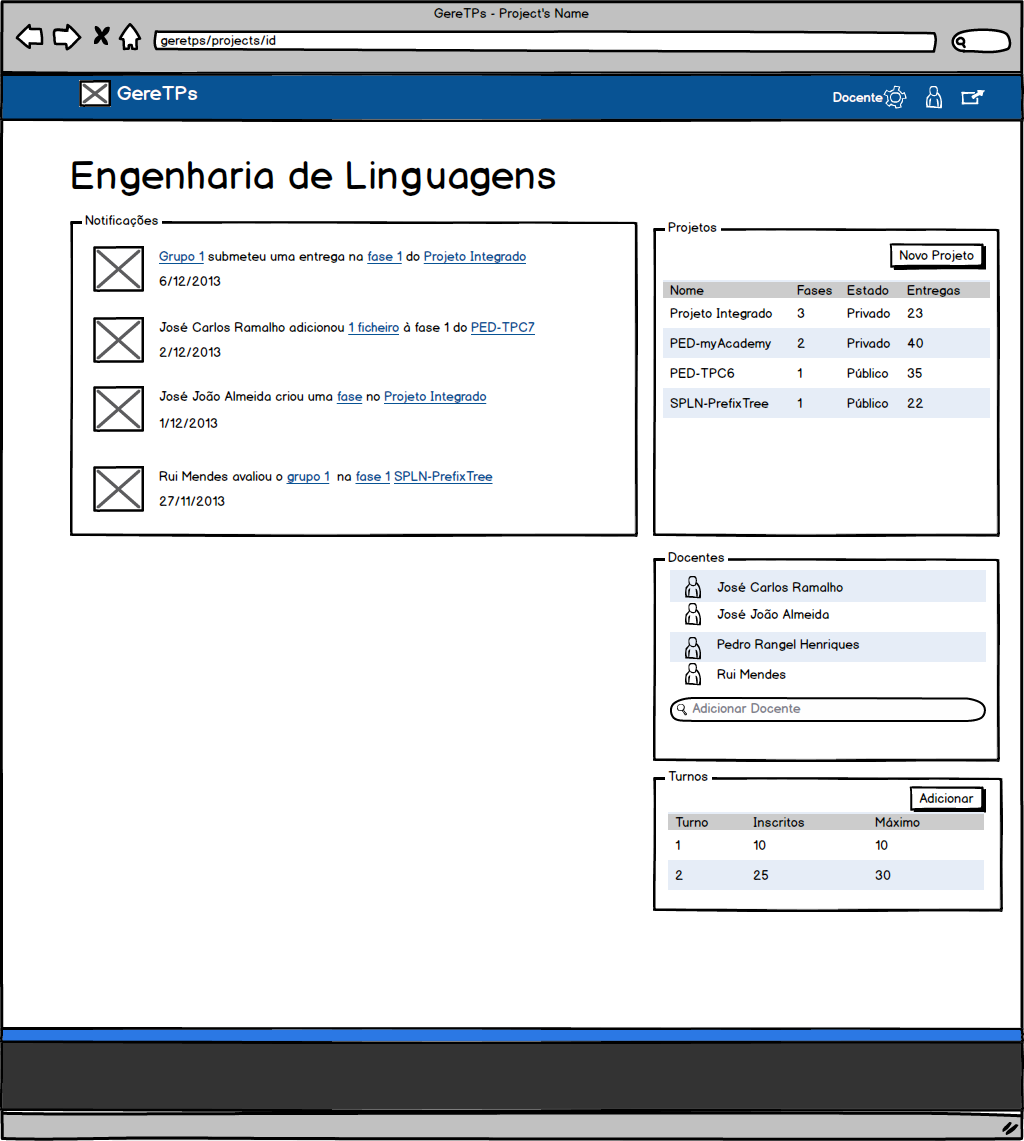
\includegraphics[width=1\textwidth]{images/prototipos/mockups/cursodocente.png}
         \caption{Painel de projeto de um aluno}
         \label{fig: cursodocente}
\end{figure}

Na paindel de pesquisa de projetos(Figura ~\ref{fig: projetospublicos}), todos os utilizadores tem acesso aos projetos públicos. Nesta página o utilizador pode filtrar uma pesquisa de forma a que o processo de pesquisa seja mais rapido. Os resultados de uma pesquisa são apresentados sob forma de blocos, desta forma, garante-se um maior aproveitamento do espaço livre da pagina.\\ 

\begin{figure}[htbp] 
        \centering
        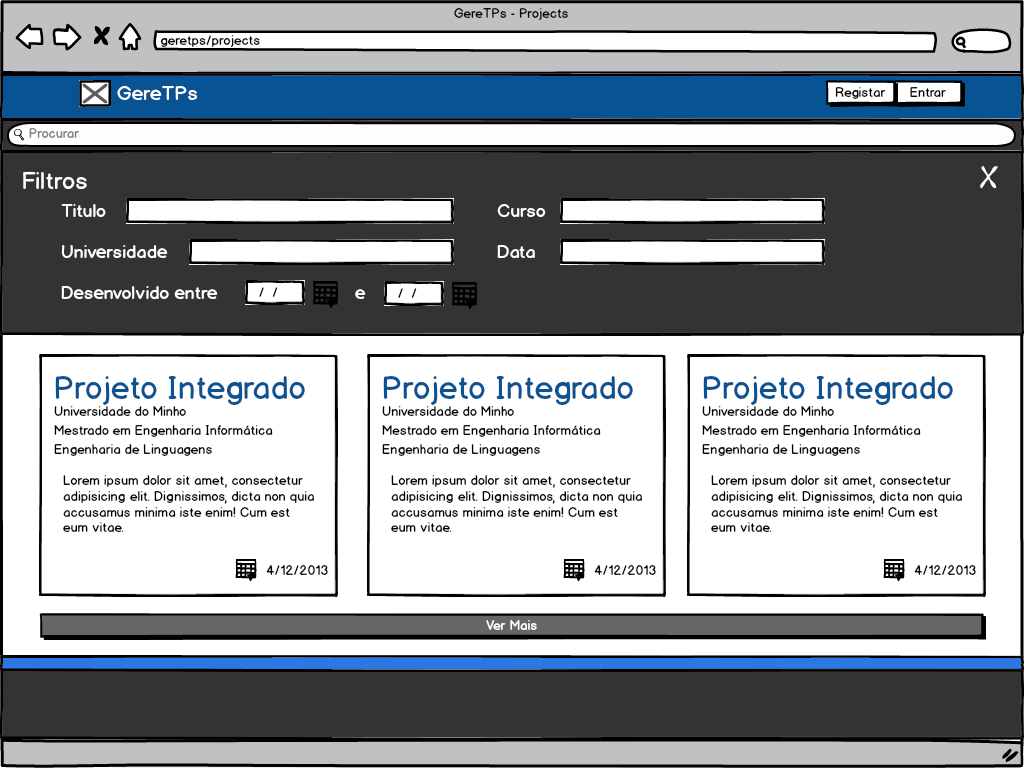
\includegraphics[width=1\textwidth]{images/prototipos/mockups/Projetos.png}
         \caption{Listagem dos projetos públicos}
         \label{fig: projetospublicos}
\end{figure}


Quando dentro de uma 

\begin{figure}[htbp] 
        \centering
        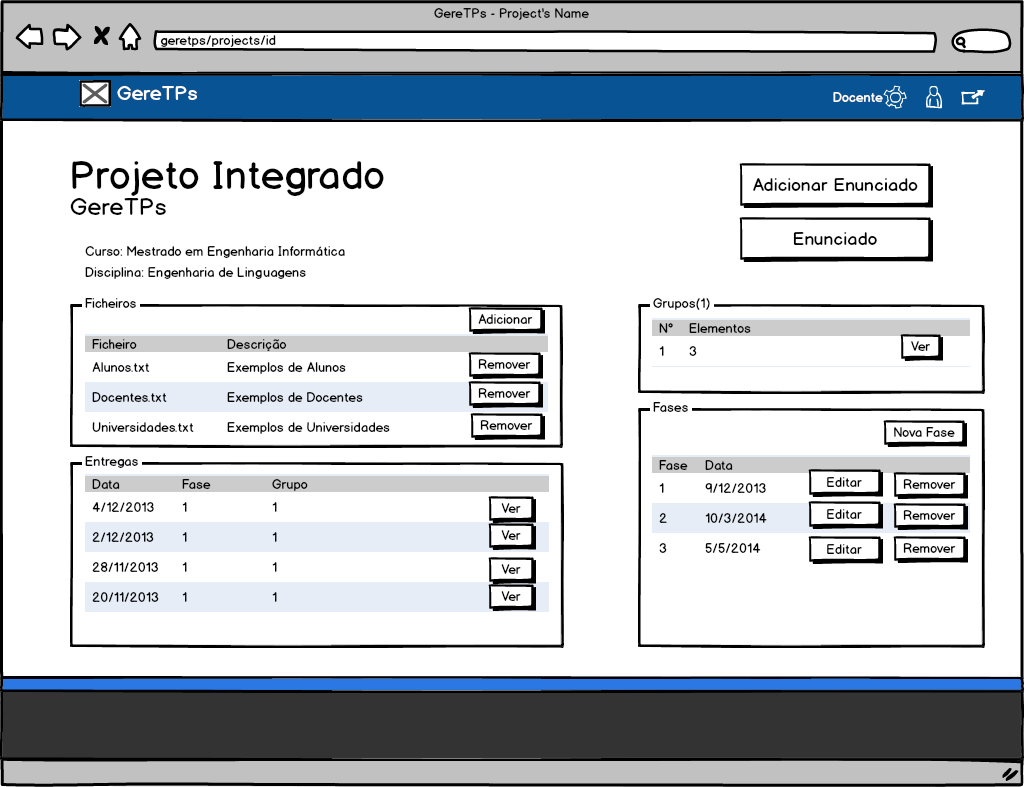
\includegraphics[width=1\textwidth]{images/prototipos/mockups/painelprojetodocente.png}
         \caption{Painel de projeto de um docente}
         \label{fig: painelprojetodocente}
\end{figure}

\begin{figure}[htbp] 
        \centering
        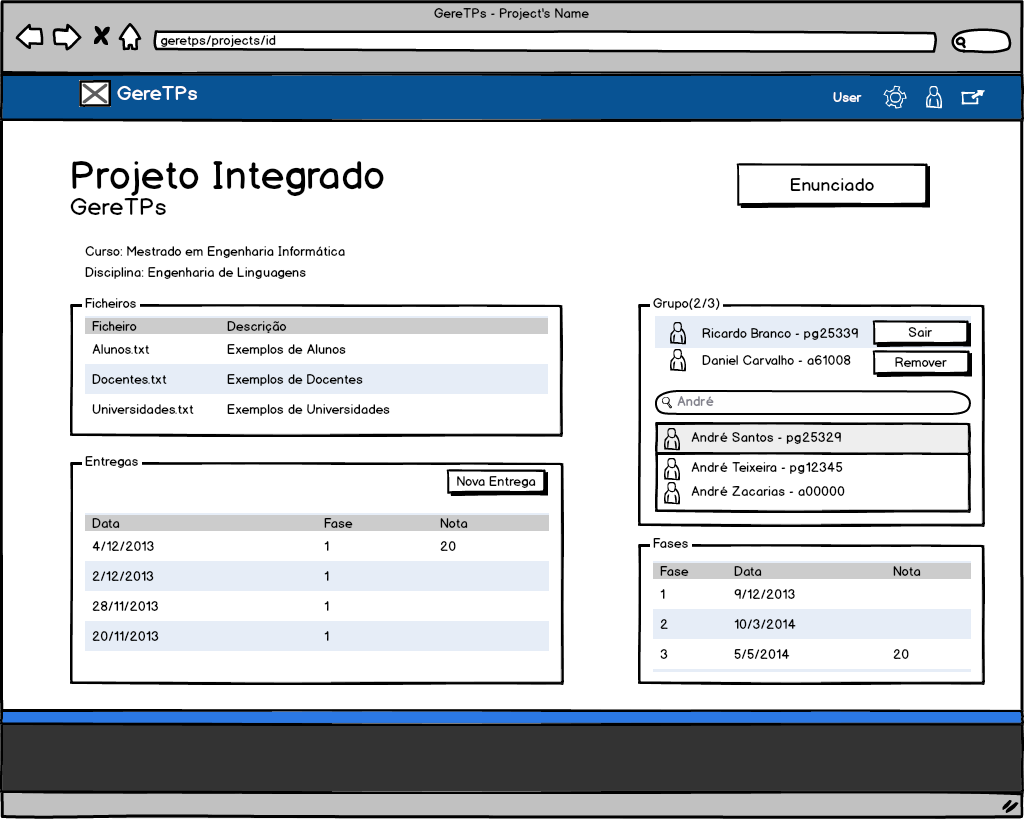
\includegraphics[width=1\textwidth]{images/prototipos/mockups/painelprojetoaluno.png}
         \caption{Painel de projeto de um aluno}
         \label{fig: painelprojetoaluno}
\end{figure}




\begin{figure}[htbp] 
        \centering
        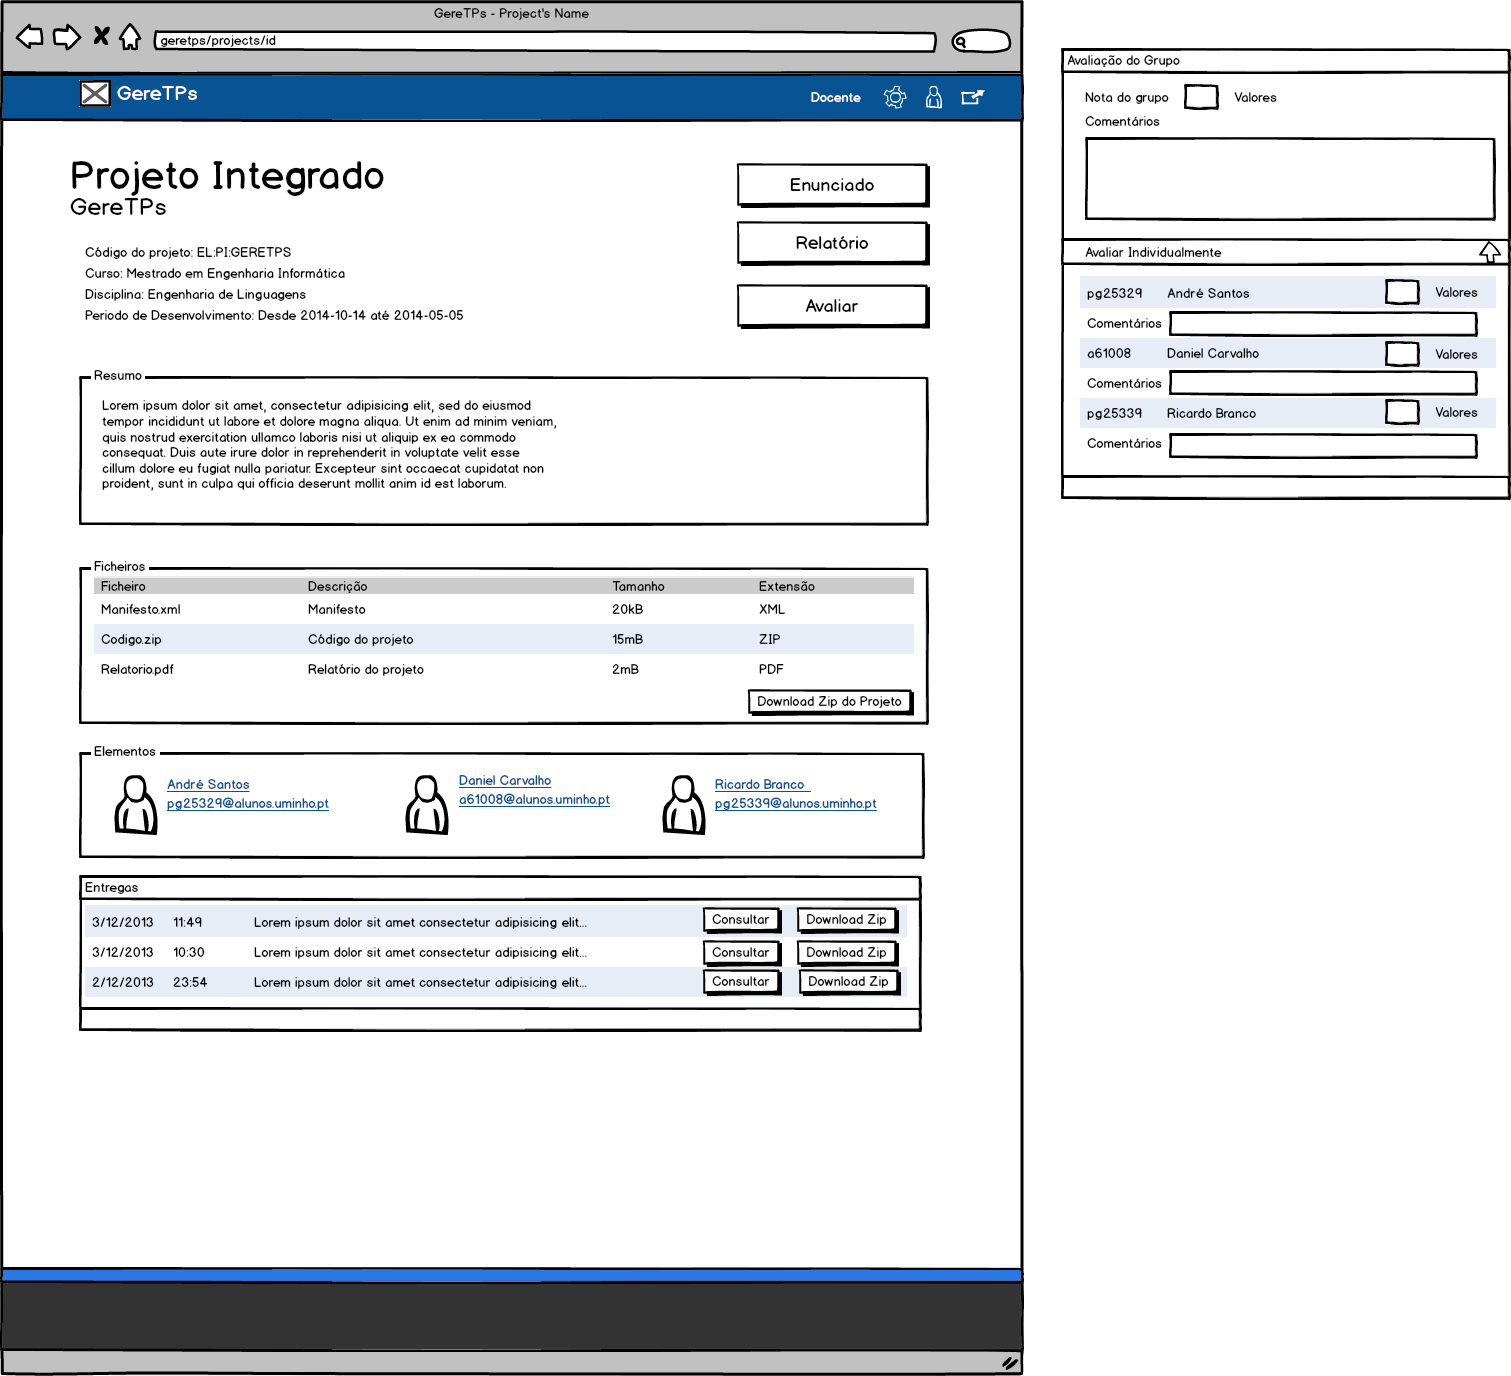
\includegraphics[width=1\textwidth]{images/prototipos/mockups/projetodocente.png}
         \caption{Entrega vista por um docente}
         \label{fig: projetodocente}
\end{figure}


\begin{figure}[htbp] 
        \centering
        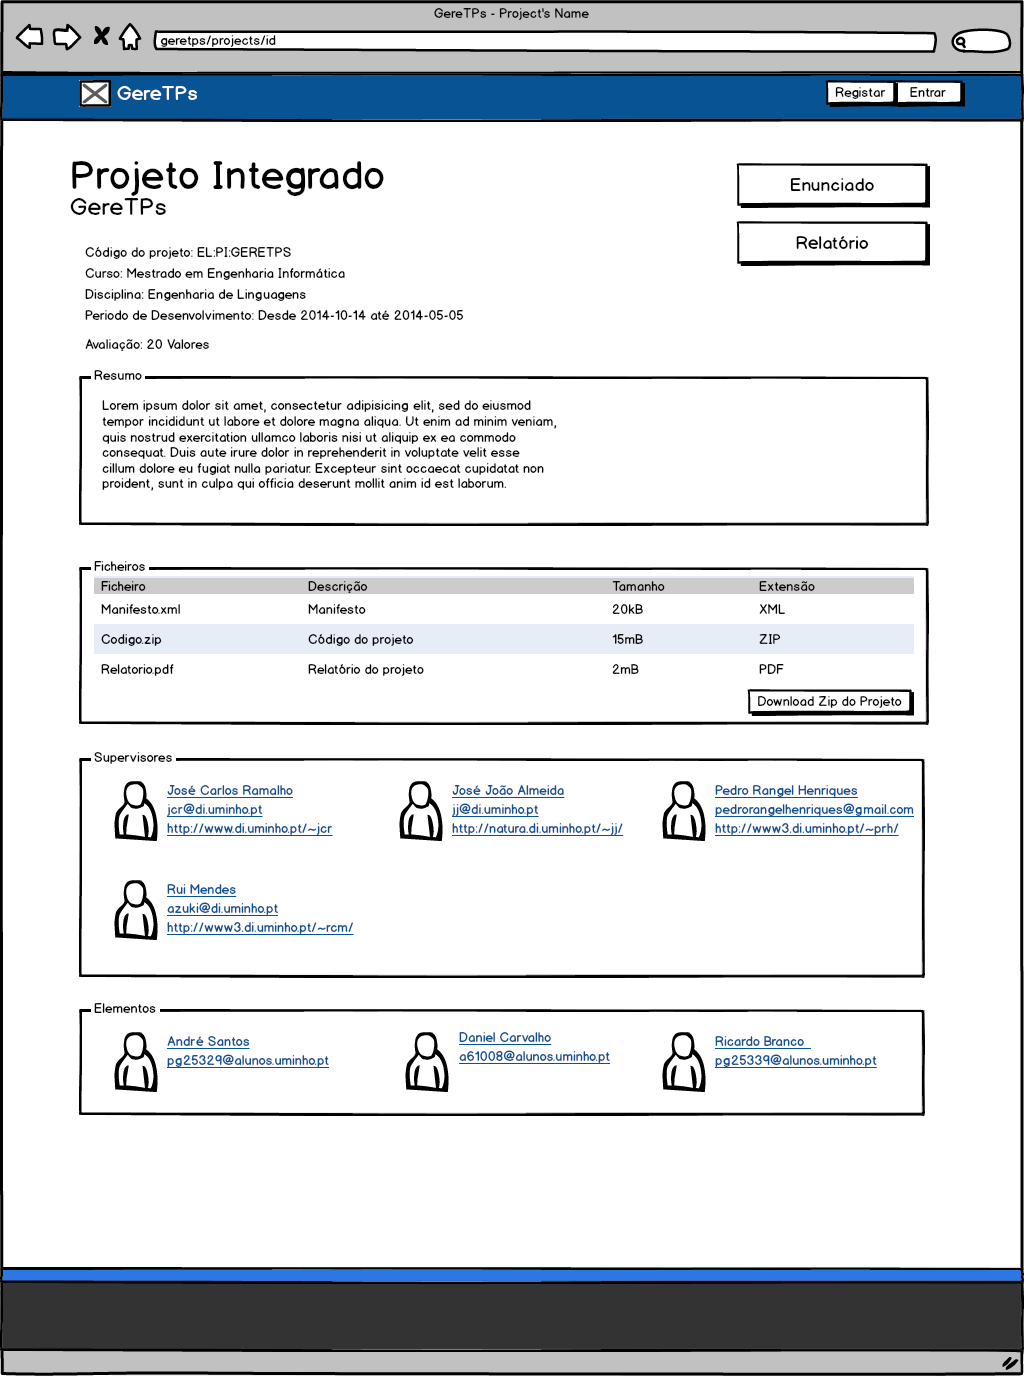
\includegraphics[width=1\textwidth]{images/prototipos/mockups/projetovisitante.png}
         \caption{Entrega vista por um visitante}
         \label{fig: projetoaluno}
\end{figure}









